\documentclass[a4paper]{report}   % To indicate fontsize, page type and document type
\setlength{\headheight}{15pt}
\usepackage[utf8]{inputenc}
\usepackage{graphicx}
\usepackage{hyphenat}
\usepackage[backend=biber, style=numeric, sorting=none]{biblatex}
\addbibresource{References.bib}


\renewcommand{\baselinestretch}{1.5}    % To make the linespacing in the document 1.5cm

\usepackage{amsmath, epsfig, graphicx, ltablex, tabularx, setspace, url, floatflt, caption, float, comment, fancyhdr, geometry, subfigure, amssymb, color, indentfirst, booktabs, array}
\usepackage[breaklinks, hidelinks]{hyperref}    % for jumping to specific page

\DeclareMathOperator*{\esup}{argmax}
%  'amsmath'   --   for [equation*]
%  'graphicx'    --   To include figures
%  'color'          --   To include texts with color and also with different fonts
%  'geometry'   --   To change page properties
%  'fancyhdr'    --   To make the pages look good by including special effects
%  'subfigure'   --   To include two figures in a single figure
% INCLUDE subfigure after fancyhdr since now it is not working because packages are not updated fully.

\geometry{left=1.25in,right=1in}
\geometry{top=1.1in,bottom=1in}       % page geometry

\setcounter{secnumdepth}{3}           % to get subsubsections numbered
\setcounter{tocdepth}{3}              % to get subsubsections in the table of contents

\begin{document}
%-----COVER PAGE-----%
\begin{titlepage}
    \begin{center}
    {\Large\sf \textbf{\textcolor[rgb]{0,0,0}{{Time Aware Food Recommender System based on Deep Learning and Graph Clustering}}}}\\[5ex]
    \vspace{0.7 cm}
    A SEMINAR REPORT\\
    submitted
    
    {\small \textcolor[rgb]{0,0,0}{\emph{By}} \\[1ex]
    {\sf \sf {\textcolor[rgb]{0,0,0}NOEL JOHN ROBERT (B20CS1147, MBT20CS090)}}} \\
    \vspace{0.5 cm}
    to
    \\
    \vspace{0.5 cm}
    \textbf{the APJ Abdul Kalam Technological University \\
        in partial fulfillment of the requirements for the award of the Degree }\\
    \vspace{0.5 cm}
    of
    \\
    \textbf{BACHELOR OF TECHNOLOGY}
    \\
    IN 
    \\
    \textit{COMPUTER SCIENCE AND ENGINEERING}
    \\
    \textbf{ December 2023}
    \vspace{0.2 cm}
    
    \begin{figure}[ht]
    \begin{center}
    \resizebox{2in}{!}{
\includegraphics{MBCETAUTONOMOUS.png}}
    \end{center}
    \end{figure}
    
    {\sf \textbf{\textcolor[rgb]{0,0,0}{DEPARTMENT OF COMPUTER SCIENCE AND ENGINEERING}}}\\[0.5ex]
    {\sf {\textcolor[rgb]{0,0,0}{MAR BASELIOS COLLEGE OF ENGINEERING \& TECHNOLOGY}}}\\[0.4ex]
    {\sf {\textcolor[rgb]{0,0,0}{(Autonomous)}}}\\[0.4ex]
    Bethany Hills, Nalanchira\\
    {\sf \textcolor[rgb]{0,0,0}{Thiruvananthapuram 15}}\\[0.5ex]
    
    \end{center}
    \end{titlepage}
    
%-----COVER PAGE-----%

%-----CERTIFICATE-----%
\thispagestyle{empty}

\setlength{\headsep}{0.4in}
\begin{center}

{\sf \textbf{\textcolor[rgb]{0,0,0}{DEPARTMENT OF COMPUTER SCIENCE AND ENGINEERING}}}\\[0.5ex]
{\sf{\textcolor [rgb]{0,0,0} MAR BASELIOS COLLEGE OF ENGINEERING \& TECHNOLOGY}}\\[0.4ex]
{\sf{\textcolor [rgb]{0,0,0}(Autonomous)}}\\[0.4ex]
Nalanchira, Thiruvananthapuram.



\end{center}


\vspace{0.15cm}
 \begin{figure}[!h]
 \begin{center}
\resizebox{3in}{!}{
\includegraphics{MBCETAUTONOMOUS.png}}
 \end{center}
 \end{figure}
\vspace{0.02cm}

\begin{center}
\textcolor[rgb]{0,0,0}{\textbf{\underline{CERTIFICATE}}} \\[1ex]
\end{center}
\par
\emph{
\textit{{This is to certify that the seminar report entitled \textbf{Time Aware Food Recommender System based on Deep Learning and Graph Clustering}  submitted by \textbf{Noel John Robert, B20CS1147, MBT20CS090} to the APJ Abdul Kalam Technological University in partial fulfillment of the requirements for the award of the Degree of {Bachelor of Technology} in {Computer Science and Engineering and Technology} is a bonafide record of the seminar work carried out by him under my guidance and supervision. This report in any form has not been submitted to any other University or Institute for any purpose}}} 



\vspace{1.0 cm}
\vspace{1.5 cm}
\vspace{1.0 cm}
\vspace{1.5 cm}


%                 Seminar Coordinator		
% \hspace{1.7 cm}	Internal Supervisor
% \hspace{1.7 cm}	Head of the Department

% \vspace{0.3 cm}

% \hspace{0.8 cm}Ms. Asha S		
% \hspace{0.8 cm} \hspace{1.5 cm} Dr. Tessy Mathew
% \hspace{0.8 cm}	\hspace{1.5 cm} Dr. Jisha John

\begin{table}[htbp]
    \centering
    \renewcommand{\arraystretch}{1.5}
    \begin{tabular*}{\textwidth}{@{\extracolsep{\fill}}lll}
        Seminar Coordinator & Internal Supervisor & Head of the Department \\
        \textbf{Ms. Asha S} & \textbf{Dr. Tessy Mathew} & \textbf{Dr. Jisha John} \\
    \end{tabular*}
\end{table}  
%-----CERTIFICATE-----%

\pagenumbering{roman}   % to get page numbers for initial pages in terms of roman numbers
%-----ACKNOWLEDGEMENTS-----%
% Acknowledgement
\chapter*{\centering Acknowledgement}
\indent First and foremost, I thank God Almighty for their divine grace and blessings in making all these possible. It is to render my heartfelt thanks and gratitude to my principal, Dr. Abraham T. Mathew, for providing the opportunity to do this seminar during the 7th semester of my B. Tech degree course.
\\
\indent Next, I would like to express my sincere gratitude to my seminar coordinator \textbf{Ms. Asha S} of the Department of Computer Science and Engineering, for her support and encouragement. I also thank my guide \textbf{Dr. Tessy Mathew} of the Department of Computer Science, for her valuable guidance and support. I also thank all the staff members of the Department of Computer Science and Engineering for providing their assistance and support. 
\\
\indent Last but not least, I thank all my friends and my family for their valuable feedback as well as their help and encouragement.
%-----ACKNOWLEDGEMENTS-----%

%-----ABSTRACT-----%
% Abstract of Seminar
\section*{\centering ABSTRACT}
\indent Recommender systems are important tools that deliver personalized content, and help recommend relevant products to customers in various domains including e-commerce, social media, and entertainment. Food recommendation systems provide an effective tool that can help users adjust their eating habits and provide a healthier diet.
\\
\indent Previous food recommender systems have shown to be effective in learning a user’s pattern by mapping previous interactions with food, but they still suffer some drawbacks, including: ingredients of food, time factor, cold start users and cold start foods, user’s community.
\\
\indent The system plans to overcome all these using a method called as “Time-aware food recommender-system based on Deep Learning and Graph Clustering [TDLGC]”\cite*{9775081}. It involves two phases: \\(i) recommendation based on users, and (ii) recommendation based on contents of food. First phase considers a similarity-matrix of the user to predict ratings and the second phase utilizes a deep-learning based clustering algorithm to group the foods into several clusters and then rating of unseen foods is predicted.
\\
\indent This  model has several novelties, such as: (i) ingredients-aware food recommender system, (ii) time-aware food recommender system, (iii) trust-aware food recommender system, (iv) community-aware food recommender system. Graph clustering is used to group nodes in a graph into clusters based on their similarity and connectivity. Edge weights are calculated using the similarities between user ratings. Deep learning uses a neural network in-order to learn the features of the users and food items. The time factor in this system is used to take into account the changes in food preferences over time.
%-----ABSTRACT-----%

\phantomsection
\tableofcontents

\clearpage

\phantomsection
\addcontentsline{toc}{chapter}{List of Figures}
\listoffigures

% \clearpage
% % \addcontentsline{toc}{chapter}{List of Tables}
% % \listoftables
% \clearpage

\phantomsection
\clearpage
\addcontentsline{toc}{chapter}{Nomenclature}
\section*{\centering Nomenclature}
\begin{enumerate}
    \item TDLGC - Time Aware Food Recommender System based on Deep Learning and Graph Clustering
    \item BERT - Bidirectional Encoder Representation from Transformer
    \item NLP - Natural Language Processing
\end{enumerate}

\newpage
\pagenumbering{arabic}
\pagestyle{fancy}                       % Sets fancy header and footer
\fancyfoot{}                            % Delete current footer settings
\fancyhead{}                            % Delete current footer settings
\rhead{TDLGC}		                    % Write seminar topic here
\lfoot{Dept: of {Computer Science and Engineering}}
\rfoot{ \thepage}
\renewcommand{\headrulewidth}{0.4pt}
\renewcommand{\footrulewidth}{0.4pt}
\renewcommand{\pagenumbering}{}

\chapter{Introduction}\label{chapter:Introduction}
% \pagenumbering{arabic}

\indent The advent of the internet and digital technologies has revolutionized the way we access information and make decisions. One area where this impact is significantly felt is in the domain of food choices. With a plethora of options available, making a healthy and personalized food choice can be overwhelming. This is where food recommender systems come into play. They aim to provide personalized food recommendations that align with the user's preferences, dietary needs, and health goals.
\\

\indent However, existing food recommender systems have several limitations. They often ignore crucial factors such as the ingredients of the food, the time factor (evolution and change in user tastes and diets over time), cold start users and foods (which have insufficient ratings or interactions), and user communities (which can improve the quality and diversity of recommendations). These limitations can lead to recommendations that are not truly personalized or beneficial to the user.
\\

Food recommender systems are categorized into three types:
\begin{itemize}
  \item Collaboratve Filtering - where items are suggested based on the preferences and behavior of similar users. Yummly is an example of this, where recipes liked by users with similar tastes are recommended.
  \item Content-based Filtering- where items are suggested after their attributes are analyzed
and matched with the user's past interaction. Foodpairing is an example, where recommendation is done based on the flavor profile of ingredients.
  \item Hybrid model - which combines the above two methods for providing a more accurate and diverse recommendations. Examples are OpenTable and HelloFresh.
\end{itemize}

\indent TDLGC is a hybrid food recommender system that combines collaborative filtering and content-based filtering approaches to address the limitations of existing systems.
\chapter{Methodology}\label{chapter:Methodology}

% \indent Citations should be included as \cite{Chen}, or \cite{Kondoz,atal} if there are more than one references to cite.

In TDLGC, the recommendation process is split into two phases:
\begin{itemize}
    \item First step is User-based rating prediction, where user's community and similarity matrices are used inorder to predict user-based ratings\cite*{9775081}.
    \item Second step is Food-based rating prediction, where food items are grouped into several clusters using a deep-learning based clustering algorithm\cite*{9775081, oulu_tdlgc} from which ratings on unseen foods are predicted.
\end{itemize}
Following these two steps, the Top-N foods are recommended\cite*{9775081} to the user.
\\
Fig 2.1\cite*{9775081, oulu_tdlgc} shows the model's conceptual framework, showcasing two distince phases: User-based rating prediction and Food-based rating prediction\cite*{9775081}. In the first phase, the model leverages user ratings along with the follower-following network inorder to generate user-user similarity matrix\cite*{9775081, oulu_tdlgc} and a trust network. Then, a graph clustering algorithm\cite*{ZHAO2021358} is used to group the users into different communities. Finally, it predicts the ratings of unseen foods for each user based on their cluster, similarity, and trust information. In the second phase, the model uses deep learning techniques to embed food ingredients into a latent space. Then, it calculates the similarity between different foods based on their embeddings. Finally, ratings on unseen foods for each user is predicted based on food similarity and historical ratings. After the two phases, the model combines the user-based and food-based rating predictions to generate a Top-N food recommendation list for each use.

\begin{figure}[htp]
    \centering
    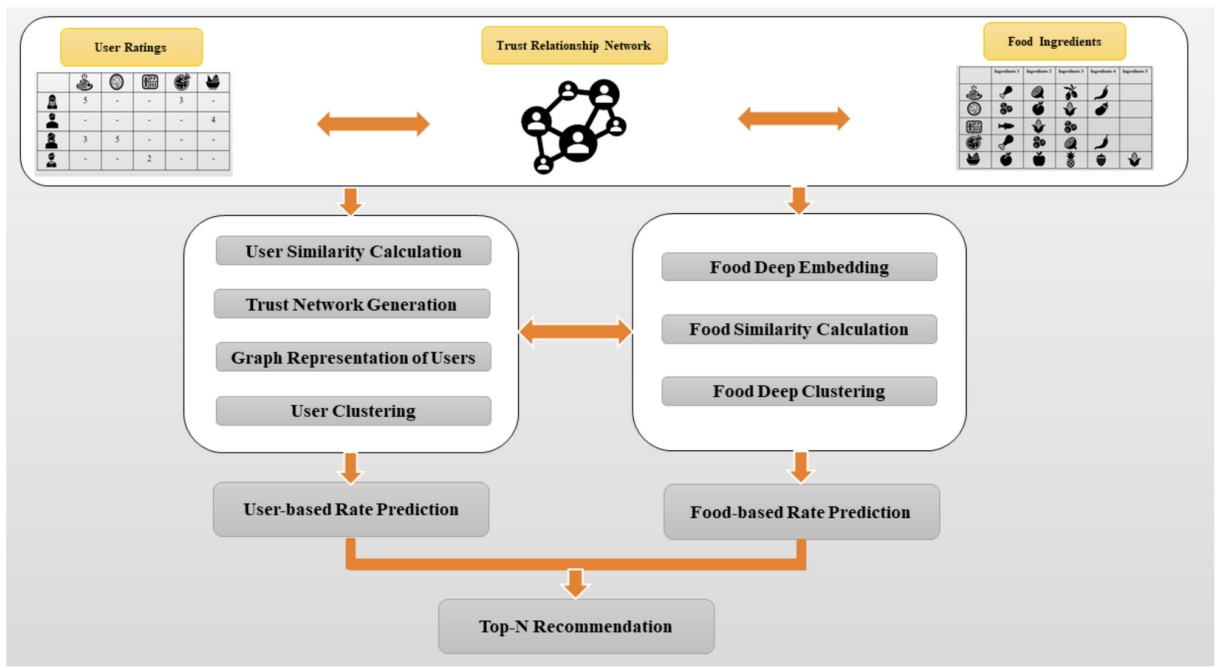
\includegraphics[width=12cm]{fig1_model_conceptual_framework.jpg}
    \caption{Conceptual framework of the model}
    \label{fig:framework}
\end{figure}

\section{User Based Rating Prediction}
\subsection{User Similarity Calculation}
Similarity measure between users is calculated using cosine similarity formula, which also takes into account ratings and time stamps of the user\cite*{9775081}.
\begin{equation*}
    sim\left({u_{i},u_{j}}\right)=\frac {a}{bc}, \tag{1}
\end{equation*}
where values of a, b, and c are found using the given formulae\cite*{9775081, oulu_tdlgc}:
\begin{align*}
    \begin{cases}
        \displaystyle a=\sum \nolimits _{k\in A_{u_{i},u_{j}}} \left({\left({r_{k}\left({u_{i}}\right)-\bar {r}\left({u_{i}}\right)}\right). \left({r_{k}\left({u_{j}}\right)}\right.}\right.
        \\
            \displaystyle \left.{\left.{\qquad \qquad -\bar {r}\left({u_{j}}\right)}\right)TW_{\left({u_{i},u_{j},k}\right)}}\right),
        \\
        \displaystyle b=\sqrt {\sum \nolimits _{k\in A_{u_{i},u_{j}}}^{}\left({\left({r_{k}\left({u_{i}}\right)-\bar {r}\left({u_{i}}\right)}\right)^{2}.TW_{\left({u_{i},u_{j},k}\right)}}\right)},
        \\[0.5pc]
        \displaystyle c=\sqrt {\sum \nolimits _{k\in A_{u_{i},u_{j}}}^{}\left({\left({r_{k}\left({u_{j}}\right)-\bar {r}\left({u_{j}}\right)}\right)^{2}.TW_{\left({u_{i},u_{j},k}\right)}}\right)}.
    \end{cases}
\end{align*}
Here, $TW_{(u_{i}, u_{j}, k)}$ represents the cumulative weights assigned to ratings of users $u_i$ and $u_j$ for food $f_k$ after factoring in time stamps of the ratings\cite*{9775081}. This weight is calculated as given in the below formula\cite*{9775081}:
\begin{equation*}
    {TW}_{\left({u_{i},u_{j},k}\right)}=e^{-\lambda \left({TP-t\left({u_{i},k}\right)}\right)}+e^{-\lambda \left({TP-t\left({u_{j},k}\right) }\right)} \tag{2}
\end{equation*}
$\lambda$ is a parameter which is controlled by the user in order to adjust the influence of time factor in calculating accumulative weight. TP indicates maximum Time Period.

\subsection{Generate Trust Network}
Trust network is a graph that represents the trust relationship among users. Some studies have shown that users who trust each other, will show profiles with similar ratings\cite*{MORADI2015462}. The assumption is made that if user $u_i$ follows user $u_j$, then there exists a trust relationship between them, or simply, user $u_i$ trusts user $u_j$. Trust network\cite*{9775081, oulu_tdlgc} is an unweighted and undirected graph TrustG(U, Tr), where U represents the set of users and Tr represents the collection of edges between users.
\\
\indent The Trust network can also be represented in the form of a weighted graph where edge weight between user $u_i$ and user $u_j$ is set to 1 if $u_i$ trusts $u_j$, else it is set to 0.

\subsection{Graph Representation of Users}
User set U is mapped onto a weighted graph G(U,E,W)\cite*{9775081, oulu_tdlgc}, where E represents set of edges linking users and W represents similarities between different users in U. To calculate the edge weights between users, a combination of Pearson correlation coefficient and the trust network that was previously obtained is utilized\cite*{9775081}, as given in the below formula:
\begin{equation*} w(u_{i},u_{j})=\alpha.Tr\left({u_{i},u_{j}}\right)+\left({1-\alpha }\right).sim\left({u_{i},u_{j}}\right). \tag{3}\end{equation*}
where Tr($u_i$,$u_j$) denotes the trust score between users $u_i$ and $u_j$.
$\alpha$ is the control parameter that adjusts contributions of trust Tr($u_i$,$u_j$) and similarity sim($u_i$,$u_j$) values.

\subsection{User Clustering}
User clustering is a technique used to group users with similar preferences in recommender systems. A graph clustering algorithm based on graph compression\cite*{ZHAO2021358} to cluster users in a large and sparse user-food rating matrix. Nodes with high similarity are iteratively merged, and edge weights are updated according to node density and influence.
\\
\indent User clustering improves perfomance of user-based rating prediction by selecting more relevant neighbors for target user.

\subsection{User-based Rating Prediction}
Prediction for ratings of food $f_k$ based on user $u_i$ is calculated as given below\cite*{9775081}:
\begin{align*} p_{k}^{u-based}\left({u_{i}}\right)\!=\!\bar {r}\left({u_{i}}\right)+\frac {\sum _{u_{j}\in C_{i}}{w(u_{i},u_{j}).\left({r_{k}\left({u_{j}}\right)\!-\!\bar {r}\left({u_{j}}\right)}\right)}}{\sum _{u_{j}\in C_{i}}\left |{w_{(}u_{i},u_{j})}\right |}. \\\tag{4}\end{align*}
where w($u_i$, $u_j$) indicates weights between users $u_i$ and $u_j$. $C_i$ represents community to which user $u_i$ belongs to.
\\
Fig 2.2\cite*{9775081} shows how user-based rating prediction is being done for a sample dataset having nine users\cite*{9775081}. User-food matrix containing rating for food given by user is used to find similarity between users. This, along with the trust network between users is used to build a graph representation of the users using which users are clustered. This is used to predict ratings of previously unseen food item with respect to each user.
\begin{figure}[htp]
    \centering
    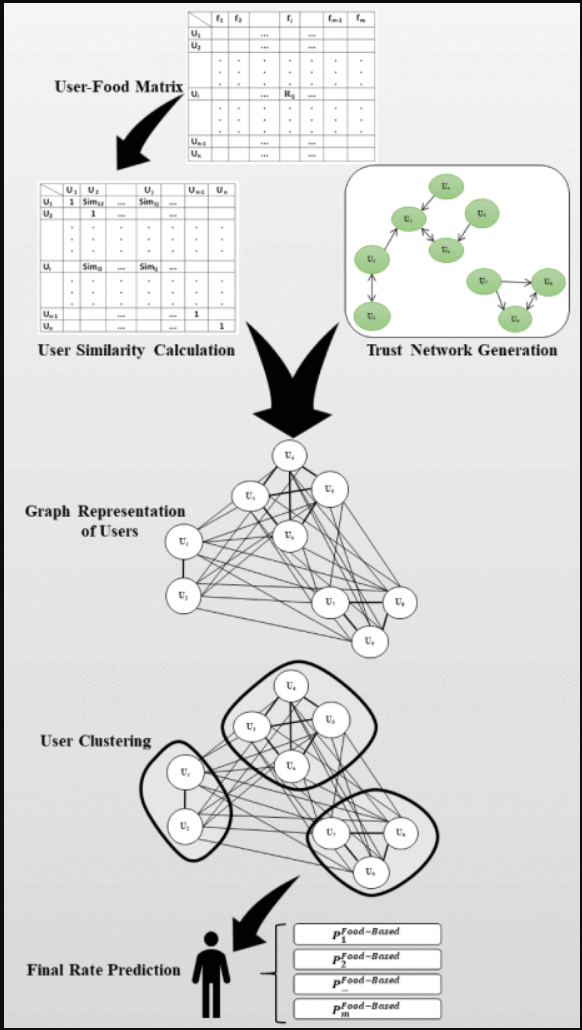
\includegraphics[scale=0.80]{overall_schema_user_based_rating_prediction.png}
    \caption{User-based rating prediction model for sample dataset with nine users}
    \label{fig:User-based rating prediction model}
\end{figure}


\section{Food Based Rating Prediction}
\subsection{Food Deep Embedding}
Food clustering based on ingredients is performed by utilizing the Bidirectional Encoder Representation from Transformer - Large (BERT-Large)\cite*{devlin2019bert}. It creates contextualized embeddings for foods. Inorder to apply Natural Langiage Processing(NLP) to food clustering, each food $f_i$ is considered as a sentence, with its ingredients $I_i$ as words\cite*{9775081, oulu_tdlgc} of the sentence.
\\
\indent Fig 2.3\cite*{9775081, oulu_tdlgc} shows how BERT is being used for food-based deep embedding\cite*{9775081}. To use Natural Language Processing (NLP) techniques for food clustering, each food $f_i$ is treated like a sentence, while its ingredients $I_i=\{ing_{\sigma(1)},ing_{\sigma(2)},ing_{\sigma(3)},\ldots,ing_{\sigma(k_i)}\}$ are treated as words in that sentence\cite*{9775081, oulu_tdlgc}. Feature extraction procedure takes the sentences(i.e. foods) and tokens(i.e. ingredients) as inputs, and generates an output JSON file - which contains simulated embeddings from different layers of BERT\cite*{9775081,devlin2019bert}. The embeddings are essentially representations of tokens as N-dimensional vectors, helping in capturing the context in which they appear.
\\
\indent The final step here invloves calculating average of all token representations within the sentence inorder to produce a contextualized representation\cite*{9775081, oulu_tdlgc}.
\begin{figure}[htp]
    \centering
    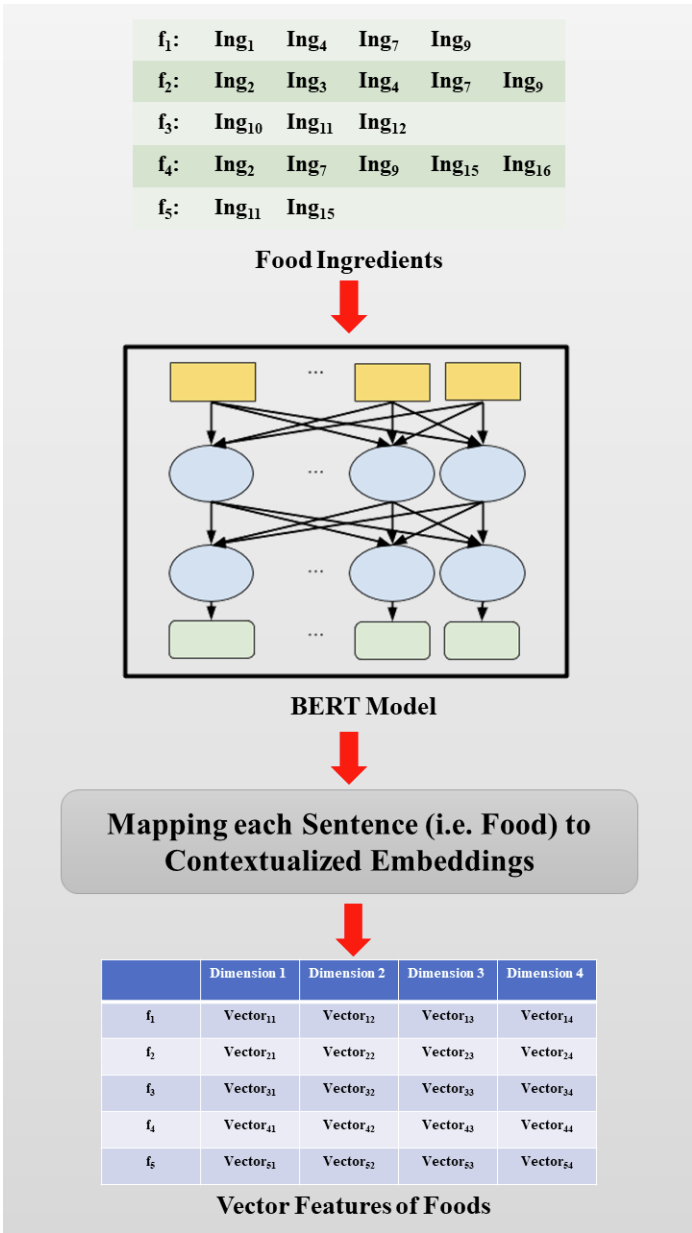
\includegraphics[scale=0.80]{overview_of_bert_based_food_embedding_method.png}
    \caption{Overview of BERT-based food embedding method}
    \label{fig:BERT-based food embedding}
\end{figure}

\subsection{Food Similarity Calculation}
By utilizing contextualized embeddings from previous step, ingredients present in a food can be identified. Similar food items are in close proximity to each other in the vector space and they are assumed to share some ingredients\cite*{9775081, oulu_tdlgc}. Euclidean distance formula is used in order to evaluate proximity between vectors of foods $f_i$ and $f_j$.
\\
\indent Let $f_i$ = \{$f_{i1}$, $f_{i2}$, $f_{i3}$, ... $f_{iL}$\} and $f_j$ = \{$f_{j1}$, $f_{j2}$, $f_{j3}$, ... $f_{jL}$\} be contextualized representation vector of food $f_i$ and $f_j$, respectively\cite*{9775081}. Similarity between $f_i$ and $f_j$ is calculated using Eucledian distance formula given as\cite*{9775081, oulu_tdlgc}:
\begin{equation*} sim\left({f_{i},f_{j}}\right)=1-\left({\sqrt {\sum _{l=1}^{L}\left({f_{il}-f_{jl}}\right)^{2}}}\right). \tag{5}\end{equation*}
where $f_{il}$ denotes l - th dimension of the contextualized representations vector of the food $f_i$.

\subsection{Food Clustering}
This step is done to group foods based on their ingredients, and overcome the data sparsity and cold start problems of collaborative filtering-based food recommender systems. It reduces distance between similar embedding vectors.
\\
\indent Deep Embedded Clustering technique is used to reduce distance between similar embedding vectors in embedding space\cite*{DBLP:journals/corr/XieGF15}. AutoEncoders and Kullback-Leiber divergence is used here to decrease the data dimensions and enhance the embedding vector representation\cite*{9775081, oulu_tdlgc}.

\subsection{Food-based Rating Prediction}
For food-based rating prediction, rating of food $f_i$ for user $u$ is calculated as:
\begin{equation*} p_{i}^{f-based}\left({u}\right)={\bar {r}}_{i}+\frac {\sum _{j\in C_{f_{i}}}{sim\left({f_{i},f_{j}}\right).\left({r_{j}\left({u}\right)-{\bar {r}}_{j}}\right)}}{\sum _{j\in C_{f_{i}}}\left |{sim\left({i,j}\right)}\right |}.\quad \tag{6}\end{equation*}
Fig 2.4\cite*{9775081, oulu_tdlgc} shows food-based rating prediction for a sample dataset having seven different food items\cite*{9775081, oulu_tdlgc}. User-food matrix and the food ingredient matrix is utilized along with BERT to perform food deep embedding. Proximity of food items in vector space is used as a factor in measuring similarity between them, and Eucledian distance formula is used to calculate this similarity. Deep Embedded Clustering technique is used to cluster the food items. Based on similarities between different foods and their previous ratings given by users, ratings of unseen foods are predicted.

\begin{figure}[htp]
    \centering
    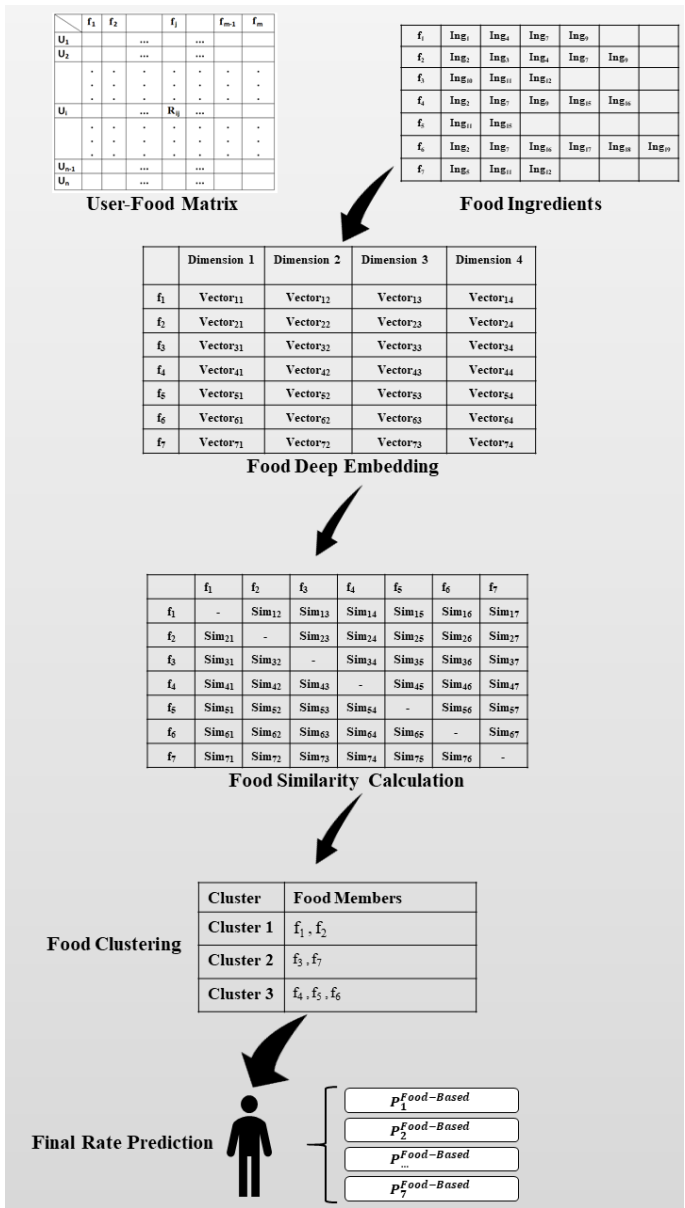
\includegraphics[scale=0.80]{overall_schema_food_based_rating_prediction.png}
    \caption{Food-based rating prediction model for sample dataset with seven users}
    \label{fig:Food-based rating prediction model}
\end{figure}


\section{Top-N Recommendation}
After performing both user-based rating prediction and food-based rating prediction, the final prediction of food $f_i$ for a user $u$ is calculated as a convex combination of these predicted values\cite*{9775081, oulu_tdlgc}. It is done by using the formula:
\begin{equation*}
    p_{i}\left({u}\right)=\beta p_{i}^{u-based}+\left({1-\beta }\right) p_{i}^{f-based}. \tag{7}
\end{equation*}
where $p_i^{u-based}$(u) and $p_i^{f-based}$(u) denotes user-based prediction and food-based prediction on food $f_i$ for user $u$ respectively\cite*{9775081, oulu_tdlgc}. Parameter $\beta$ controls whether user-based or food-based prediction value has a higher priority in final outcome. A higher value of $\beta$ means user-based rating prediction was given a higher priority in influencing the final outcome, while a lower value means food-based rating prediction was given higher priority.
\chapter{Conclusion} \label{chapter:Conclusion}

\indent The development and implementation of a robust and efficient food recommender system is a timely and relevant endavour in today's world. This is primarily due to the increasing health consciousness among people. As individuals strive for personalized dietary recommendations that align with their health goals, dietary restrictions and taste preferences, a system that can properly cater to these individuals is much needed.
\\
\indent The digital age has ushered in an era of information overload. The vast amount of food-related information widely available online can be overwhelming for many users. In such scenarios, recommender systems work as a valuable tool in helping the users to navigate through this plethora of information and discover new tools which align with their needs and goals.
\\
\indent Personalization is an important aspect which underscores the need for such a system. They significantly help in enhancing user satsifaction and engagement with the platform. This increases user retention and makes the system very beneficial for users.
\\
\indent In conclusion, TDLGC addresses several challenges faced by currently existing systems and meet the current needs and expectations of users for personalized and health-conscious food recommendations. It can greatly contribute to promotion of healthy eating habits of its users, thereby making it a valuable tool for the users.

%-----include as many chapters as needed-----%

%-----REFERENCES-----%
\phantomsection
\addcontentsline{toc}{chapter}{References}
\setcounter{biburllcpenalty}{7000}
\setcounter{biburlucpenalty}{8000}
\printbibliography[title={References}]
%-----REFERENCES-----%

\end{document}